\documentclass[a4paper]{article}

% Import some useful packages
\usepackage[margin=0.5in]{geometry} % narrow margins
\usepackage[utf8]{inputenc}
\usepackage[english]{babel}
\usepackage{hyperref}
\usepackage{minted}
\usepackage{amsmath}
\usepackage{xcolor}
\usepackage{graphicx}
\definecolor{LightGray}{gray}{0.95}

\title{Peer-review of assignment 5 for \textit{INF3331-peterek}}
\author{oleksako, {oleksako@uio.no} \\
 		martimj, {martimj@uio.no} \\
		andhols, {andhols@uio.no}}

\begin{document}
\maketitle

\section{Review}\label{sec:review}

The assignment was tested on an UiO machine (Red Hat Enterprise Linux Server 6.8) and Python 3.5.2.

%%%%%%%%%%%%%%%%%%%%%%%%%%%%%%%%%%%%%%%%%%%%%%%%%%%%%%%%%%
\subsection*{General feedback}
The code is clean and well structured. The names for functions and variables are very intelligible. All this makes the code easy to read.

What is good is that the program uses argparse to process the input arguments, which makes the processing of arguments very pleasant and simple at the same time. We can advise to have slightly more comments.

%%%%%%%%%%%%%%%%%%%%%%%%%%%%%%%%%%%%%%%%%%%%%%%%%%%%%%%%%%
\subsection*{Assignment 5.1: Syntax highlightning}

The program work as expected with the provided example (hello.py). However, it behaves weird with the examples in the tasks 5.2 and 5.3. All the lines of a similar type either disappear or become substituted with the first line of its type (see on the examples below). This might be a system specific, and behaves differently on a Windows machine. Furthermore, as was explained on piazza forum, the program should be able to process enclosed blocks, which it does not do. 

\begin{minted}[bgcolor=LightGray, linenos, fontsize=\footnotesize]{python}
#!/usr/bin/env python3
# Comments dissapear or become Comment 1 everywhere
# Comment 2 
from typing import List
import argparse
# Comment 3 

def equalize(arr1: List, arr2: List, element=" some string in here"):
    if size_orig < size_mod:
        for i in range(size_mod - size_orig):
            arr1 += [element]
    elif size_orig > size_mod:
        for_function():

    return arr1, arr2
# Comment 4 with an enclosed 

definition to(test function definitioni):

""""""

def compare(orig_file: str, mod_file: str):
        """ comparing lines of two files, printing and writing to file.
                
        """
        while a == True and b == False:
            orig_file = orig_file.split("\n")
            mod_file = mod_file.split("\n")

        orig_file, mod_file = equalize(orig_file, mod_file)
        with open("diff_output.txt", 'a') as out:
                for line_o, line_mod in zip(orig_file, mod_file):
                        if line_o == line_mod:
                                line = "0 " + line_o
                                out.write(line + '\n')
                                print("0", line_o)
                        elif line_o != line_mod:
                                line = "- " + line_o
                                line2 = "+ " + line_mod
                                out.write(line + '\n')
                                out.write(line2 + '\n')
                                print("-", line_o)
                                print("+", line_mod)

\end{minted}

\begin{figure}
  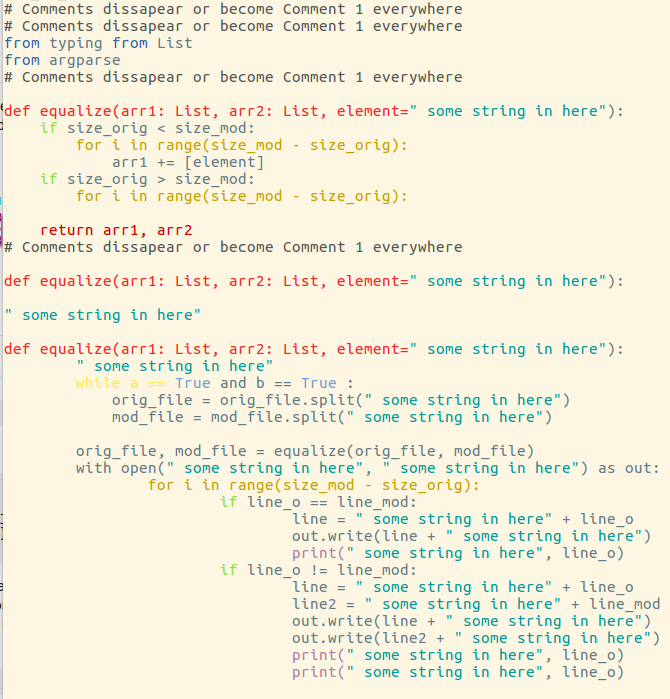
\includegraphics[scale=0.5]{feedback.png}
\end{figure}


%%%%%%%%%%%%%%%%%%%%%%%%%%%%%%%%%%%%%%%%%%%%%%%%%%%%%%%%%%
\subsection*{Assignment 5.2:  Python syntax} \label{sec:assignment5.2}

It was hard to test parts 5.2, 5.3 and 5.4 because of the implementation of "higlighter.py" from the part 5.1, which incorrectly substituted lines. However, these mistakes should not be considered as drawbacks of part 5.2, 5.3 and 5.4.

As for the regex implementation there just one thing to mention. 
In many places "*" (zero or more) is better to change on "+" (one or more):

\begin{minted}[bgcolor=LightGray, linenos]{python}
      "\b(def\s*.*\(.*\):)": def
\end{minted}

\begin{minted}[bgcolor=LightGray, linenos]{python}
      "\b(def\s+.*\(.+\):)": def
\end{minted}

With "zero or more", regex wrongly catches words even if they are just a starting part of other words. For example "definition to(test function definitioni):" will be treated as def. Same applies to the other regex rules.

%%%%%%%%%%%%%%%%%%%%%%%%%%%%%%%%%%%%%%%%%%%%%%%%%%%%%%%%%%
\subsection*{Assignment 5.3: Syntax for your favorite language}
We have assessed files for the programming language C in this section. Similar to the previous part, instead of 'zero or more' it is better to use 'one or more'. Other than that, all looks good.

%%%%%%%%%%%%%%%%%%%%%%%%%%%%%%%%%%%%%%%%%%%%%%%%%%%%%%%%%%
\subsection*{Assignment 5.4:  Syntax for your second favorite language}
We have assessed files for the programming language Java in this section. In many regexes are missing the leading 'backslash b'. In all those cases the sought-for words become highlighted even if they occur at the end of bigger words. For example, in word "myclass", "mint", "sherif", the endings "class", "int" and "if" will be colorized. Besides that, all seems to work as expected.

%%%%%%%%%%%%%%%%%%%%%%%%%%%%%%%%%%%%%%%%%%%%%%%%%%%%%%%%%%
\subsection*{Assignment 5.5: superdiff}
As was mentioned at the piazza forum, the best way to implemet the task would be using "Longest common subsequence". Your implementation often mistakenly treat blocks without changes as if each line there was first deleted and then inserted.

%%%%%%%%%%%%%%%%%%%%%%%%%%%%%%%%%%%%%%%%%%%%%%%%%%%%%%%%%%
\subsection*{Assignment 5.6: Coroling diff}

The coloring looks good.

\bibliographystyle{plain}
\bibliography{literature}

\end{document}